\documentclass[17pt]{extarticle}
\usepackage{tikz}

\begin{document}
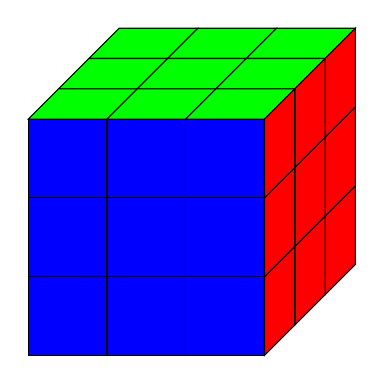
\begin{tikzpicture}
\foreach \x in {0,1,2}
{
    \foreach \y in {0,1,2}
    {
        \path[draw,fill=blue] (\y,\x,3) -- (\y+1,\x,3) -- (\y+1,\x+1,3) -- (\y,\x+1,3)--cycle; % breite,länge,tiefe
    }   

    \foreach \y in{0,1,2}
    {   
        \path[draw,fill=green] (\y,3,\x+1) --(\y+1,3,\x+1) -- (\y+1,3,\x) -- (\y,3,\x)--cycle;
    }

    \foreach \y in{0,1,2}
    {   
        \path[draw, fill=red] (3,\y,\x+1) -- (3,\y,\x) -- (3,\y+1,\x) -- (3,\y+1,\x+1)--cycle; % breite,länge,tiefe
    }
}
\end{tikzpicture}
\end{document}